\chapter{Einführung \LaTeX}
\LaTeX~ermöglicht das Erstellen eines einheitlichen Dokuments mit nur wenigen Grundeinstellungen. Es erlaubt jedoch auch eine benutzerdefinierte Formatierung bis hin zum kleinsten Detail eines Dokumentes. Anhand des kurzen Einführungskapitels soll auf die wichtigsten Grundfunktionen eingegangen werden.

\section{Grundformatierung}
Im Textbearbeitungsprogramm \LaTeX~wird zwischen folgenden Untergliederungsstufen unterschieden:
\begin{itemize}
	\item \verb|\chapter{Kapitel}|
	\item \verb|\section{Unterkapitel}|
	\item \verb|\subsection{Unterunterkapitel}|
	\item \verb|\subsubsection{Unterunterunterkapitel}|
	\item \verb|\paragraph{Paragraph}|
	\item \verb|\subparagraph{Unterparagraph}|
\end{itemize}

Eine Untergliederung ist jedoch nur bis zur \verb|\subsection{Titel}| sinnvoll. In Einzelfällen kann eine weitere Gliederungsstufe \verb|\subsubsection{Titel}| notwendig werden. Diese wird dann aber nichtmehr im Inhaltsverzeichnis aufgelistet.\\

Abstände werden grundsätzlich von \LaTeX~selbst gesetzt und müssen nicht extra hinzugefügt werden. Sollte es dennoch so sein das man Abstände erzwingen möchte so funktioniert das entweder mit \verb|\newline| oder \verb|\\|.

\section{Aufzählungen}
Aufzählungen können ganz einfach mit
\begin{verbatim}
\begin{itemize}
   \item Aufzählungspunkt 1
   \item Aufzählungspunkt 2
\end{itemize}
\end{verbatim}
eingefügt werden.\pagebreak

Das Ergebnis sieht dann wie folgt aus:
\begin{itemize}
	\item Aufzählungspunkt 1
	\item Aufzählungspunkt 2
\end{itemize}
Wird \verb|itemize| mit \verb|enumerate| ausgetauscht so werden statt Aufzählungspunkten entsprechende Zahlen ausgegeben. Die Nummerierung beginn in der Regel bei \verb|1.|.

\section{Abbildungen}
Abbildungen können entweder mit dem im Editor vorhandenen Assistenten eingefügt oder manuell über folgende Zeilen:

\begin{verbatim}
\begin{figure}[H]
	\centering
	\includegraphics[width=0.6\linewidth]{fh_campus}
	\caption{\acs{fh} wird zum Campus St. Pölten~\cite{fhcampus_link}}
	\label{fig:fhcampus}
\end{figure}
\end{verbatim}

Das Ergebnis sieht dann wie folgt aus:
\begin{figure}[H]
	\centering
	\includegraphics[width=0.6\linewidth]{Figures/fh_campus}
	\caption{\acs{fh} wird zum Campus St. Pölten~\cite{fhcampus_link}}
	\label{fig:fhcampus}
\end{figure}
Mit \verb|[width=0.6\linewidth]| wird beispielsweise die Breite des Bildes auf 60\% der Gesamttextbreite festgelegt. \verb|\caption{Bildunterschrift}| definiert eine Bildunterschrift, \verb|\label{fig:fhcampus}| ermöglicht das Referenzieren des Bildes im Text.

Beispielsweise könnte die Referenzierung wie folgt aussehen:

\textit{In der Abbildung \ref{fig:fhcampus} ist das neue Campusgebäude der FH St. Pölten zu sehen.}
\pagebreak

\section{Tabellen}
Tabellen erweitern die Komplexitätsstufe der manuellen Erstellung erheblich. Für das grobe Layout empfiehlt sich grundsätzlich der Tabellenassistent. Für eine feinere beziehungsweise spezielle Formatierung muss händisch nachgearbeitet werden.

\begin{table}[H]
	\begin{tabular}{|c|c|c|c|c|c|}
		\hline 
		\multirow{2}{*}{\sffamily{\textbf{Wert}}} & \sffamily{\textbf{Metallschicht}} & \multicolumn{2}{c|}{\multirow{2}{*}{\sffamily{\textbf{Toleranzbereich}}}} & \multirow{2}{*}{\sffamily{\textbf{Messwert}}} & \multirow{2}{*}{\sffamily{\textbf{Im Toleranzbereich}}} \\
		& \sffamily{\textbf{Toleranzfarbe}} & \multicolumn{2}{c|}{} & & \\
		\thickhline
		$510~\Omega$ & Braun & $515.1~\Omega$ & $504.9~\Omega$ & $506~\Omega$ & \textcolor{green}{$\checkmark$} \\ 
		\hline
		$4.7~k\Omega$ & Braun & $4747~\Omega$ & $4653~\Omega$ & $4650~\Omega$ & {\Large \textcolor{red}{$\times$}} \\ 
		\hline 
		$100~k\Omega$ & Braun & $101~k\Omega$ & $99~k\Omega$ & $100~k\Omega$ & \textcolor{green}{$\checkmark$} \\ 
		\hline 
	\end{tabular}
	\caption{Wertetabelle verschiedener Metallschichtwiderstände}
	\label{tab:metallschichwiderstaende}
\end{table}

Auch hier kann die Tabelle wieder im Text referenziert werden.

\textit{Aus der Tabelle \ref{tab:metallschichwiderstaende} geht klar heraus das sich der $4.7k\Omega$ Widerstand nicht im Toleranzbereich befindet.}

\section{Mathematische Formeln}
Recht beliebt ist auch die Möglichkeit mathematische Funktionen, Rechenschritte und Co direkt in \LaTeX~zu dokumentieren. Dazu unterscheidet man zwischen folgenden Definitionen:
\begin{description}
	\item[Inline] Hier wird die Formel direkt in der Zeile eingefügt. $ c = \sqrt{a^2 + b^2} $
	\item[displaymath] Die Formel wird hierbei in einer neuen Zeile mittig eingefügt. \begin{displaymath}
	c = \sqrt{a^2 + b^2}
	\end{displaymath}
	\item [equation] Auch hier wird die Formel mittig in einer separaten Zeile eingefügt, weiters erscheint am Rand eine fortlaufende Nummer. Diese kann wie bei Bildern oder Tabellen bekannt im Text referenziert werden.
	\begin{equation} \label{eq:quadratwurzel}
	c = \sqrt{a^2 + b^2}
	\end{equation}
\end{description}

\textit{Die Länge der Hypotenuse entspricht der Quadratwurzel aus der Summe der Kathetenquadrate, mathematisch ausgedrückt folgt daraus die Formel \ref{eq:quadratwurzel}.}

\section{Interessante Packages}
Mithilfe diverser Pakete lassen sich recht schön verschiedenste Objekte in \LaTeX~einbinden. Für diverse Anwendungsfälle existieren eigene Pakete, eine Internetrecherche führt mit den richtigen Suchbegriffen am schnellsten zur idealen Lösung.
\subsection*{tikz}
Mit \verb|tikz| lassen sich eine Vielzahl an Diagrammen im 2D als auch 3D Raum erstellen. 
\begin{figure}[H]
	\centering
	\begin{tikzpicture}
	\pie[sum=auto, radius=3, text=pin, color={yellow, cyan, red, magenta},after number=\%]
	{
		46.6/Chrome,
		24.6/Internet Explorer,
		20.4/Firefox,
		8.4/Other
	}
	\end{tikzpicture}
	\caption{Verwendete Browser laut Musterstudie XY}
\end{figure}

\begin{figure}[H]
	\centering
	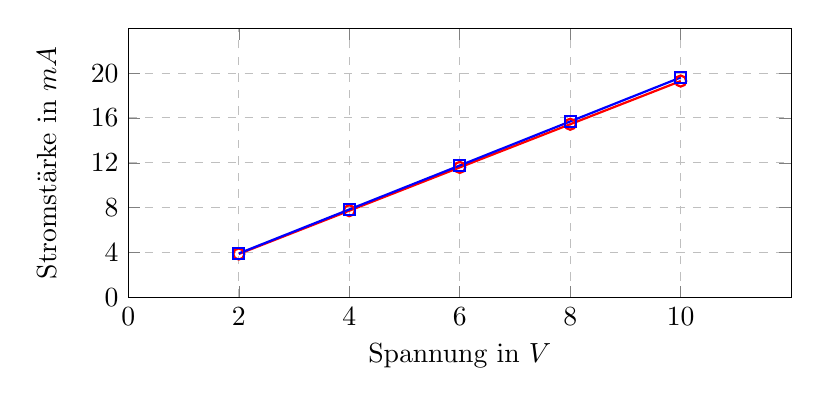
\begin{tikzpicture}
	\begin{axis}[width=10cm,height=5cm,ylabel shift = .2cm,
	xlabel={Spannung in $V$},
	ylabel={Stromstärke in $mA$},
	xmin=0, xmax=12,
	ymin=0, ymax=24,
	xtick={0,2,4,6,8,10},
	ytick={0,4,8,12,16,20},
	log ticks with fixed point,
	%legend style={at={(0.5,-0.1)},anchor=north},
	legend columns=-2,
	legend entries={gemessen, berechnet},
	legend to name=named,
	ymajorgrids=true,
	xmajorgrids=true,
	grid style=dashed,
	/pgf/number format/.cd,
	use comma,
	1000 sep={},
	]
	
	\addplot [color=red, thick, mark=o]  coordinates {
		(2,3.87)
		(4,7.73)
		(6,11.59)
		(8,15.44)
		(10,19.29)
	};
	
	\addplot [color=blue, thick, mark=square] coordinates {
		(2,3.92)
		(4,7.84)
		(6,11.76)
		(8,15.69)
		(10,19.61)
	};
	\end{axis}
	\end{tikzpicture}
	\ref{named}
	\caption{Linearität der Stromstärke -- $510~\Omega$}
\end{figure}

\subsection*{listings}
Für die Dokumetation des Quellcodes steht das Paket \verb|listings| zur Verfügung.

Mit \verb|\lstinputlisting{Datei}| kann eine ganze Datei einfach in die Dokumentation eingebunden werden.

\lstset{language=Python,caption={Primzahlenevaluierung, \lstname},label=DescriptiveLabel}
\begin{codeblock}
	\lstinputlisting{Code/Exercise_Task_1.py}
\end{codeblock}

\section{Verzeichnisse}
Eine anständige und ordentliche Dokumentation benötigt selbstverständlich entsprechende Verzeichnisse. Sei es ein Abbildungsverzeichnis \verb|\listoffigures|, ein Tabellenverzeichnis \verb|\listoftables|, Codeverzeichnisse \verb|\lstlistoflistings| oder ein Literaturverzeichnis. \LaTeX~erstellt diverse Verzeichnisse unabhängig davon ob sie benötigt werden oder nicht, eingebunden werden sie mit den im Text angeführten Befehlen. Das Literaturverzeichnis benötigt ein wenig Eigeninitiative. Abhängig von den entsprechenden Quellen sind andere Definitionen zu wählen.